\documentclass[12pt]{report}
\usepackage[a4paper]{geometry}
\usepackage[myheadings]{fullpage}
\usepackage{fancyhdr}
\usepackage{lastpage}
\usepackage{graphicx, wrapfig, subcaption, setspace, booktabs}
\usepackage{babel}
\usepackage[T1]{fontenc}
\usepackage[font=small, labelfont=bf]{caption}
\usepackage{fourier}
\usepackage[protrusion=true, expansion=true]{microtype}
\usepackage{algorithm}
\usepackage{algorithmic}
\usepackage{algpseudocode}
\usepackage{sectsty}
\usepackage{url, lipsum}
\usepackage{tgbonum}
\usepackage{hyperref}
\usepackage{xcolor}

\newcommand{\HRule}[1]{\rule{\linewidth}{#1}}
\onehalfspacing
\setcounter{tocdepth}{5}
\setcounter{secnumdepth}{5}
\begin{document}
{\fontfamily{cmr}\selectfont
\title{ \normalsize
		\\ [0.005cm]
		\HRule{0.002pt} \\
		\LARGE \textbf{\uppercase{SOEN 6011- SOFTWARE  ENGINEERING PROCESSES\\
		PROJECT DELIVERABLE 3\\}
		\HRule{1pt} \\ [0.1cm]
		\normalsize \
		\begin{center}
    
\includegraphics[ height=5cm, width=10cm]{Image/Untitled.png}
\end{center}\vspace*{4\baselineskip}}
		}
\date{August 2, 2019}

\author{Jemish Kishor Paghadar (40080723)\\https://github.com/Jemish27121997/SOEN6011\_Function\_Implementation\\
			Concordia University, Montreal}

			
\maketitle
\tableofcontents
\pagebreak

\section{Problem 5}
\subsection{Source Code Review for Function Gamma($\Gamma$)}
\noindent The main focus of this section is to provide a brief summary of the source code review made on the Gamma function $f(x) = \Gamma(x)$.

\noindent\textbf{Introduction : }Gamma function($\Gamma \left( x \right)$) is a commonly used extension of the factorial function to complex numbers.\\ Lets define f be the Gamma Function from A to B, therefore A is the domain and B is the  co-domain of the Gamma Function.\\ 
\noindent\textbf{Domain of function : }includes all complex numbers and the positive integer.\\
\noindent\textbf{Co-domain of function : }When a in A is a positive integer, then the gamma function is related to the factorial function  $\Gamma(a) = (a-1)!$ \\
 When a in A for complex numbers with a positive real part, then the ${\displaystyle \Gamma (a)=\int _{0}^{\infty }x^{a-1}e^{-x}\,dx.}$

\newline
\noindent\textbf{Source Code Review : }
Source Code review is systematic examination (sometimes referred to as peer review) of computer source code. It is intended to find mistakes overlooked in the initial development phase, improving the overall quality of software. Code review aims to warranty the quality of a system program by reviewing someone else code to give him/her a feedback of our review of by receiving feedback from someone else that performed a review on one$'$s code.
This activity could be performed manually as well as automatically by using
sophisticated tools already available in the market.
Viewing someone else code helps to improve the quality of the system program,
generate new ideas, solve problems and increase the sense of mutual
responsibility. Although direct discovery of quality problems is often the
main goal, code reviews are usually performed to reach a combination of
goals.
Reviews can be done in various forms such as pair programming, informal walkthroughs, and formal inspections.
\newline
\indent The review of the source code for the Gamma function is carried out manually as well as automatically. For the manual review, the general programming style
rules were followed, some of these standards include Coding conventions (naming conventions, commenting conventions, indentation), Object oriented principles such as encapsulation, information hiding, cohesion and coupling, Refactoring and Restructuring techniques etc. 
For the automated review, the source code review tool PMD Eclipse was used, this
tool was selected among other ones because it provides a complete violations
summary of the reviewed code. Apart from this, the details given for any violation is described in a clear, straightforward form and it is very easy to understand and navigate.

\clearpage
\subsection{Manual Source Code Review for Function Gamma($\Gamma$)}

For the manual review for this function, the general programming style rules were followed, some of these standards include Coding conventions, Object oriented principles, Refactoring and Restructuring techniques etc. It can be done by evaluating source code against these standards.  \\
\newline
Coding conventions are a set of prescriptive rules that pertain
to how code is to be written, including :\\
\noindent
\textbf{File organization : }how code is distributed between files,
and organized within each file.\\
\textbf{Indentation : }how particular syntactical elements are to
be indented in order to maximize readability. For example the keywords like if, while, for and switch must be followed by a space.\\
\textbf{Comments : }how to consistently and efficiently use
comments to help program understandability. For example, use of Javadoc comments.\\
\textbf{Declarations : }what particular syntax to use to declare
variables, data structures, classes, etc. in order to
maximize code readability.\\
\textbf{Naming : }how to give names to various named entities in
a program as to convey meaning embedded into the
names. For example, Class names should be a noun and begin with a
capital letter or Method names should be verbs and begin with a lower case
letter.\\
\textbf{Refactoring : }It is a disciplined technique for
restructuring an existing body of code, altering its internal
structure without changing its externally observable
behavior. \\
\textbf{Cohesion and Coupling : }Coupling is the measure of the degree of interdependence between the modules and Cohesion is a measure of the degree to which the elements of the module are functionally related. A good software design must have high cohesion and low coupling.
\newline\newline
There are more standards to assure a correct programming style. However, the ones mentioned above were considered the most relevant for this approach to review code. Manual review for Gamma function is described below.
\begin{itemize}
    \item \textbf{MainFrame.java}\\
    \textbf{File Organization :}Code is not properly distributed between files. There is only one mainframe file which includes functional code and configuration code as well.There should be two files for better organization and understandability.\\
    \textbf{Indentation : }Source code is correctly indented.\\
    \textbf{Comments : }Effectively and Efficiently use of comments which is easy to understand.\\
    \textbf{Declaration : }Properly declared code which is easy to read.\\
    \textbf{Naming : }Proper use of Names on the class and method elements.\\
\textbf{Refactoring : }Refactoring can be applied to improve code quality. In one method called arithmeticOperation on the line 110, duplicate conditional fragment can be moved outside expression. \\
\textbf{Cohesion and Coupling : }Code is written with high cohesion and low coupling which is very easy to modify.

    
    \item \textbf{CalcultorTests.java}\\
    \textbf{Indentation : } Source code is correctly indented.\\
    \textbf{Comments : }Effectively and Efficiently use of comments which is easy to understand.\\
    \textbf{Declaration : }Properly declared code which is easy to read.\\
    \textbf{Naming : }Proper use of Names on the class and method elements.\\
\textbf{Refactoring : }Code is already refactored. \\
\textbf{Cohesion and Coupling : }Code is written with high cohesion and low coupling which is very easy to modify.
\end{itemize} 

\clearpage
\subsection{Automated Source Code Review for Function Gamma($\Gamma$)}

For the automated source code review the PMD source code review tool was used as a plug-in for eclipse IDE.\\\\
\textbf{The Eclise PMD plug-in }\\
It integrates the well-known source code analyzer PMD 6.16.0 into the Eclipse IDE.\\
\textbf{Analyse : }Everytime you save your work, eclipse-pmd scans your source code and looks for potential problems like possible bugs and suboptimal, duplicate, dead or overly complicated code.\\
\textbf{Locate : }When eclipse-pmd finds problems it highlights those in your editor so you can fix them right away. Discovered problems are also logged in the Eclipse Problems View.
\textbf{Fix : }Where possible, eclipse-pmd offers quick fixes that automatically fix the problems. These quick fixes can be used to fix a single problem or all occurrences in your entire code base.

The tool showed some violations on the code that will be briefly described below.

\begin{figure}[h!]
    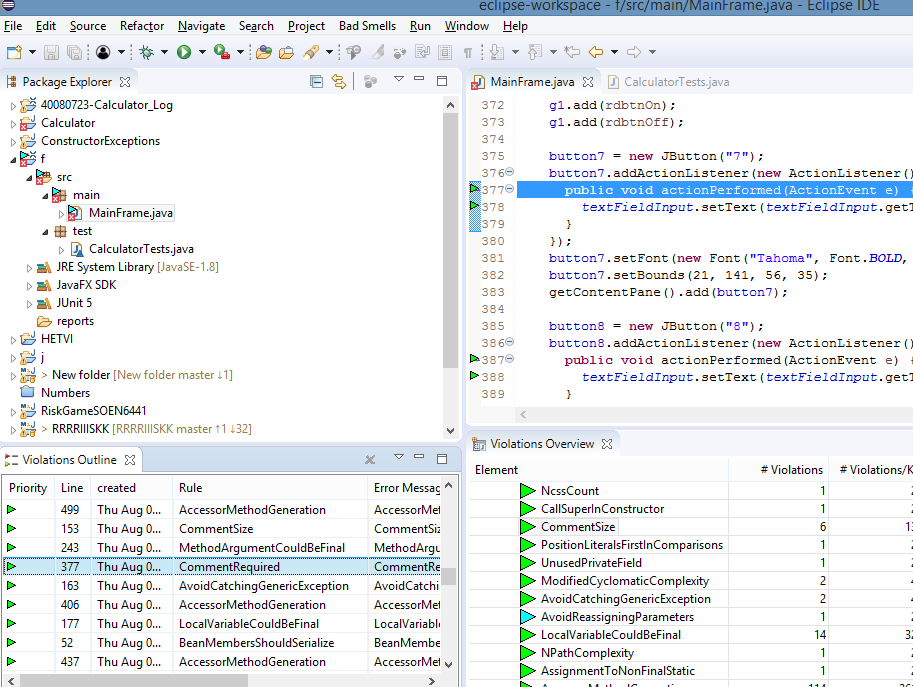
\includegraphics[width=16cm, height=10cm]{Image/automaticReview1.png}
    \caption{CommentRequired violation for class MainFrame}
\end{figure}
\clearpage
\indent A summary of the PMD tool that was executed on class MainFrame as shown in figure 1. The PMD tool classify the violations by color, green color stands for urgent violations, red means blocker violations, blue ones are critical violations, pink are important violations and navy ones are warnings.
\newline\\From the review, it an be seen that comment is missing for the public method on the line 377 of MainFrame.java file and it suggests that comment is required to increase understandability of source code.
\newline

\begin{figure}[h!]
    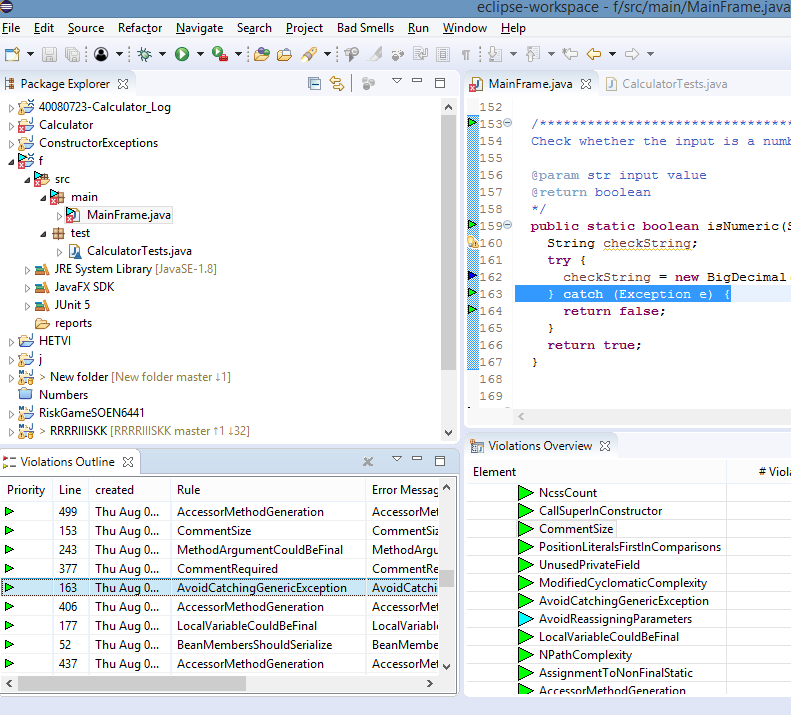
\includegraphics[width=16cm, height=10cm]{Image/automaticReview2.png}
    \caption{Catching General Exception violation for class MainFrame}
\end{figure}
\newline
\indent From the figure 2, it is inferred that there is use of generic Exception in catch clause on the line 163 of MainFrame.java file. The consequence of the generic catch clause is that logging is limited because catch doesn't know the specific exception being caught which contradicts the purpose of using catch blocks.
\noindent
\clearpage
As shown in figure 3, the string literal "Tahoma" appears 23 times in this file and it suggests to avoid using duplicate literal many times.\newline
\begin{figure}[h!]
    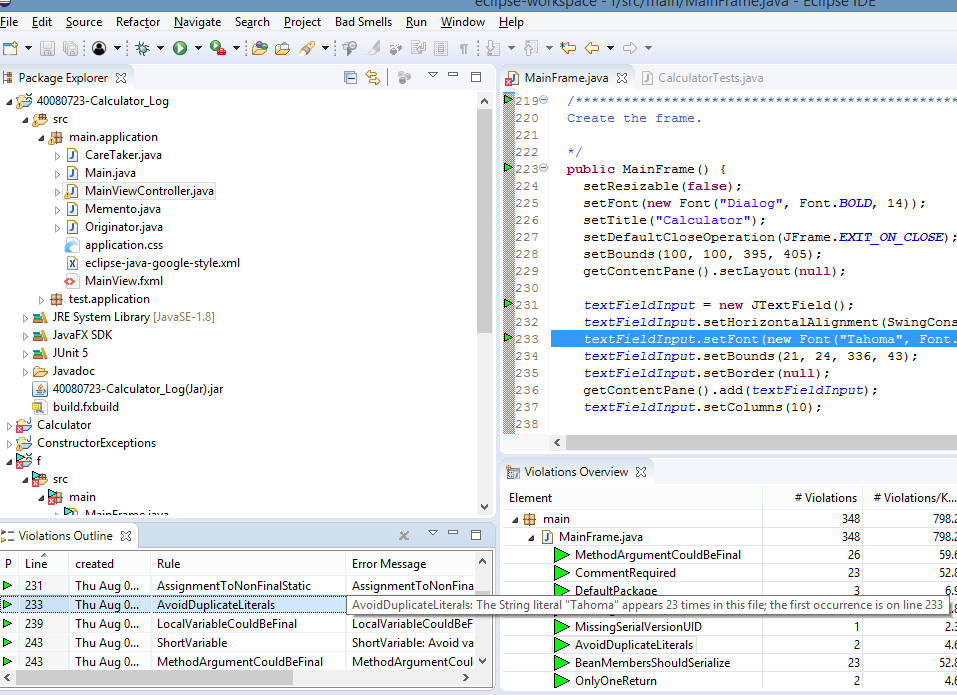
\includegraphics[width=16cm, height=10cm]{Image/automaticReview3.png}
    \caption{Duplicate literals violation for class MainFrame}
\end{figure}
\clearpage
\section{Problem 7}
\subsection{Test Cases Analysis for Function $f(x)=ab^x$}
\noindent The main focus of this section is to provide a brief summary of the test case analysis carried out on the function $f(x) = ab^x$.
\newline
\noindent\textbf{Introduction : }
This function involves an exponent. This exponent is represented with a variable, and its base is represented with constant value. Let $f(x) = ab^x$ be an exponential function where ''b'' is a constant, the exponent is the independent variable, the coefficient ''a'' is called the initial value of the function , and ''f(x)'' represent the dependent variable.
\\
\newline
\noindent\textbf{Test Case Analysis : }A test case is a set of instructions on ''HOW'' to validate a particular test objective/target, which when followed will tell us if the expected behavior of the system is satisfied or not.
Functional testing is a type of software testing which is used to verify the functionality of the software application, whether the function is working according to the requirement specification. In functional testing, each function tested by giving the value, determining the output, and verifying the actual output with the expected value. Functional testing performed as black-box testing which is presented to confirm that the functionality of an application or system behaves as we are expecting. It is done to verify the functionality of the application. It concentrates on:\\
\textbf{Basic Usability : }Functional Testing involves the usability testing of the system. It checks whether a user can navigate freely without any difficulty through screens.\\
\textbf{Accessibility : }Functional testing test the accessibility of the function.\\
\textbf{Mainline function : }It focuses on testing the main feature.\\
\textbf{Error Condition : }Functional testing is used to check the error condition. It checks whether the error message displayed.\\
These are the following steps that I have followed to perform for test case analysis:
\begin{itemize}
    \item There is a need to understand the software requirement.
    \item Identify test input data.
    \item Compute the expected outcome with the selected input values.
    \item Execute test cases.
    \item Comparison between the actual and the computed result.
\end{itemize}

For this function $f(x)=ab^x$ implementation, three test cases were created that cover general as well as common input validations. These tests cases are traceable to initial requirements.
From the figure, it can be seen that there are no any test cases that directly test the function itself but all test cases are running properly without any failure.\newline
\begin{figure}[h!]
    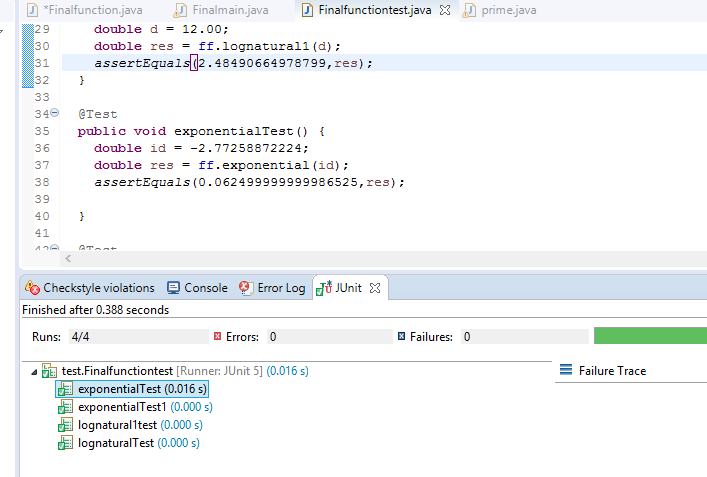
\includegraphics[width=16cm, height=10cm]{Image/testReview1.png}
    \caption{Successful Execution of each test cases}
\end{figure}
\newline
For validating this function a set of different inputs will be passed to each unit test, the results will be posted on a summary table.
\newline
\noindent The test cases to be analyzed are :\\
\textbf{lognaturalTest()} which tests the natural logarithm value for an input given within the range of 0 to 1.\\ 
\noindent\textbf{lognatural1Test()} which tests the natural logarithm value for an input given above 1. 
\textbf{exponentialTest()} which tests the exponential value for any input.
\newline
\newline
The summary tables for the test cases are described below which compares the actual output with the expected output.\\
\clearpage
\noindent
\textbf{Test Case method : lognaturalTest()} which validates the natural logarithm value for an input given within the range of 0 to 1. From the table, it can be seen that all the inputs are validated properly and giving the accurate results of natural logarithm.\\

\begin{center}
\begin{tabular}{ |c|c|c|c| } 
\hline
\textbf{Input} & \textbf{Expected Result} & \textbf{Actual Result} & \textbf{Status} \\
\hline
0.5 & -0.6931471805599445 & -0.6931471805599445 & Passed \\ 
\hline
0.65 & -0.4307829160924539 & -0.4307829160924539 & Passed \\ 
\hline
\end{tabular}
\end{center}
\noindent\newline\textbf{Test Case method : lognatural1Test()} which validates the natural logarithm value for an input above 1. From the below table, it can be seen that all the inputs are validated successfully and this method is also giving the accurate results of natural logarithm.\\

\begin{center}
\begin{tabular}{ |c|c|c|c| } 
\hline
\textbf{Input} & \textbf{Expected Result} & \textbf{Actual Result} & \textbf{Status} \\
\hline
12.00  & 2.48490664978799 & 2.48490664978799 & Passed \\ 
\hline
50.5 & 3.9219733362812597 & 3.9219733362812597 & Passed \\ 
\hline
\end{tabular}
\end{center}

\newline\noindent\textbf{Test Case method : exponentialTest()} which validates the exponential value for any input. All the inputs are validated successfully without any failure.\\

\begin{center}
\begin{tabular}{ |c|c|c|c| } 
\hline
\textbf{Input} & \textbf{Expected Result} & \textbf{Actual Result} & \textbf{Status} \\
\hline
-2.77258872224 & 0.062499999999986525 & 0.062499999999986525 & Passed \\ 
\hline
100 & 2.6881171418161336E43 & 2.6881171418161336E43 & Passed \\ 
\hline
2.718 & 15.149991940878161 & 15.149991940878161 & Passed \\ 
\hline
\end{tabular}
\end{center}
\newline
\newline
Therefore, from the test cases analysis, it is clear that all the test cases are successfully executing without any failure.


\section{Version Control System}
To have a common repository for all project files available and updated remotely, distributed version control system(Git) is maintained.
\\Clone the repository from below link\\
https://github.com/Jemish27121997/SOEN6011\_Function\_Implementation.git

\section{Acknowledgments}
I would like to thank Professor Pankaj Kamthan and his great group of teaching assistants for the material and guidance. I would also like to thank my teammates Jingya Pan and Koteswara Rao Panchumarthy for giving access to their source code for review.

\begin{thebibliography}{9}
\bibitem{pmd}
\url{https://www.javatips.net/blog/pmd-in-eclipse-tutorial}
\bibitem{wiki}
\url{https://en.wikipedia.org/wiki/Code_review}
\bibitem{testing}
\url{https://www.javatpoint.com/functional-testing}
\bibitem{Git}
\url{https://github.com/Jemish27121997/SOEN6011_Function_Implementation}
\end{thebibliography}
}
\end{document}

